\subsection{Electrons and Photons}\label{sec:eg_reco}
Electrons and photons share many of the same reconstruction and identification algorithms because, with the exception of an electron's track, the two particle leave similar signatures in the detector. Both particles are expected to be contained within the ECAL, and have almost identical showering properties. In this section, reconstruction for electron and photon ($\eg$) objects will be described together, with differences highlighted where necessary.

\subsubsection{Electron and Photon Identification}\label{sec:eg_id}

Background sources for prompt electrons include photon conversions, hadrons misidentified as electrons, and secondary electrons from semileptonic decays of b or c quarks. Background sources for prompt photons are primarily secondary photons from light neutral mesons ($\pi^0$ and $\eta$). Using variables related to the isolation and shower shape of the electrons and photons, multivariate (MVA) discriminators are trained to separate real electrons and photons from these background sources~\cite{CMS:2020uim}. Additional tracker-related variables are also used for the identification of electrons.

The isolation variables are constructed by considering a cone of $\dR<0.3$ around the \eg candidate and summing the \pt of the charged hadrons (\Ich), photons (\Iph), and neutral hadrons (\In) inside the cone. As is done for \IPF, a pileup correction is applied in these sums, and these variables are useful for discriminating against backgrounds originating from jets. Another important variable is the ratio of energy of associated HCAL clusters to the supercluster energy (H/E), which is expected to be lower for \eg objects than for hadrons.

The shower shape variables exploit differences in the showering of prompt \eg objects from photons from neutral hadron decays, which are expected to have a wider profile on average. One such variable is $\sigma_{i\eta i\eta}$, which is the standard deviation of the shower in $\eta$ in terms of the absolute number of crystal cells~\cite{CMS:2020uim}. Another important variable is \RNINE, which is a measure of how localized the energy deposit is, and is defined as the ratio of the energy of the $3\times3$ cell grid surrounding the SC seed to the energy of the SC. For electrons, variables related to the compatibility of the track with the SC are also used which include the differences between the energy, $\eta$ and $\phi$ of the electron, measured by the track and the SC.

These discriminating variables are combined into single discriminators using BDTs. This is done separately for electron and photons and the BDTs are trained on simulated DY + jets and $\gamma$ + jets events for electrons and photons respectively. In both cases, the dependence on $\eta$ and \ET is included, either by introducing these variables as inputs to the BDT, or by training several BDTs in different bins of $\eta$ and \ET. The performance of these algorithms as measured by simulation for 2017 is shown in \cref{fig:eg_id_performance}. Two working points are defined: WP90 and WP80, corresponding to signal efficiencies of about 90\% and 80\% respectively and physics analyses are left to choose which point to use based upon their level of background. 

\begin{figure}
  \includegraphics[width=0.49\textwidth]{Figures/Detector/CMS/electron_id_performance.pdf}
  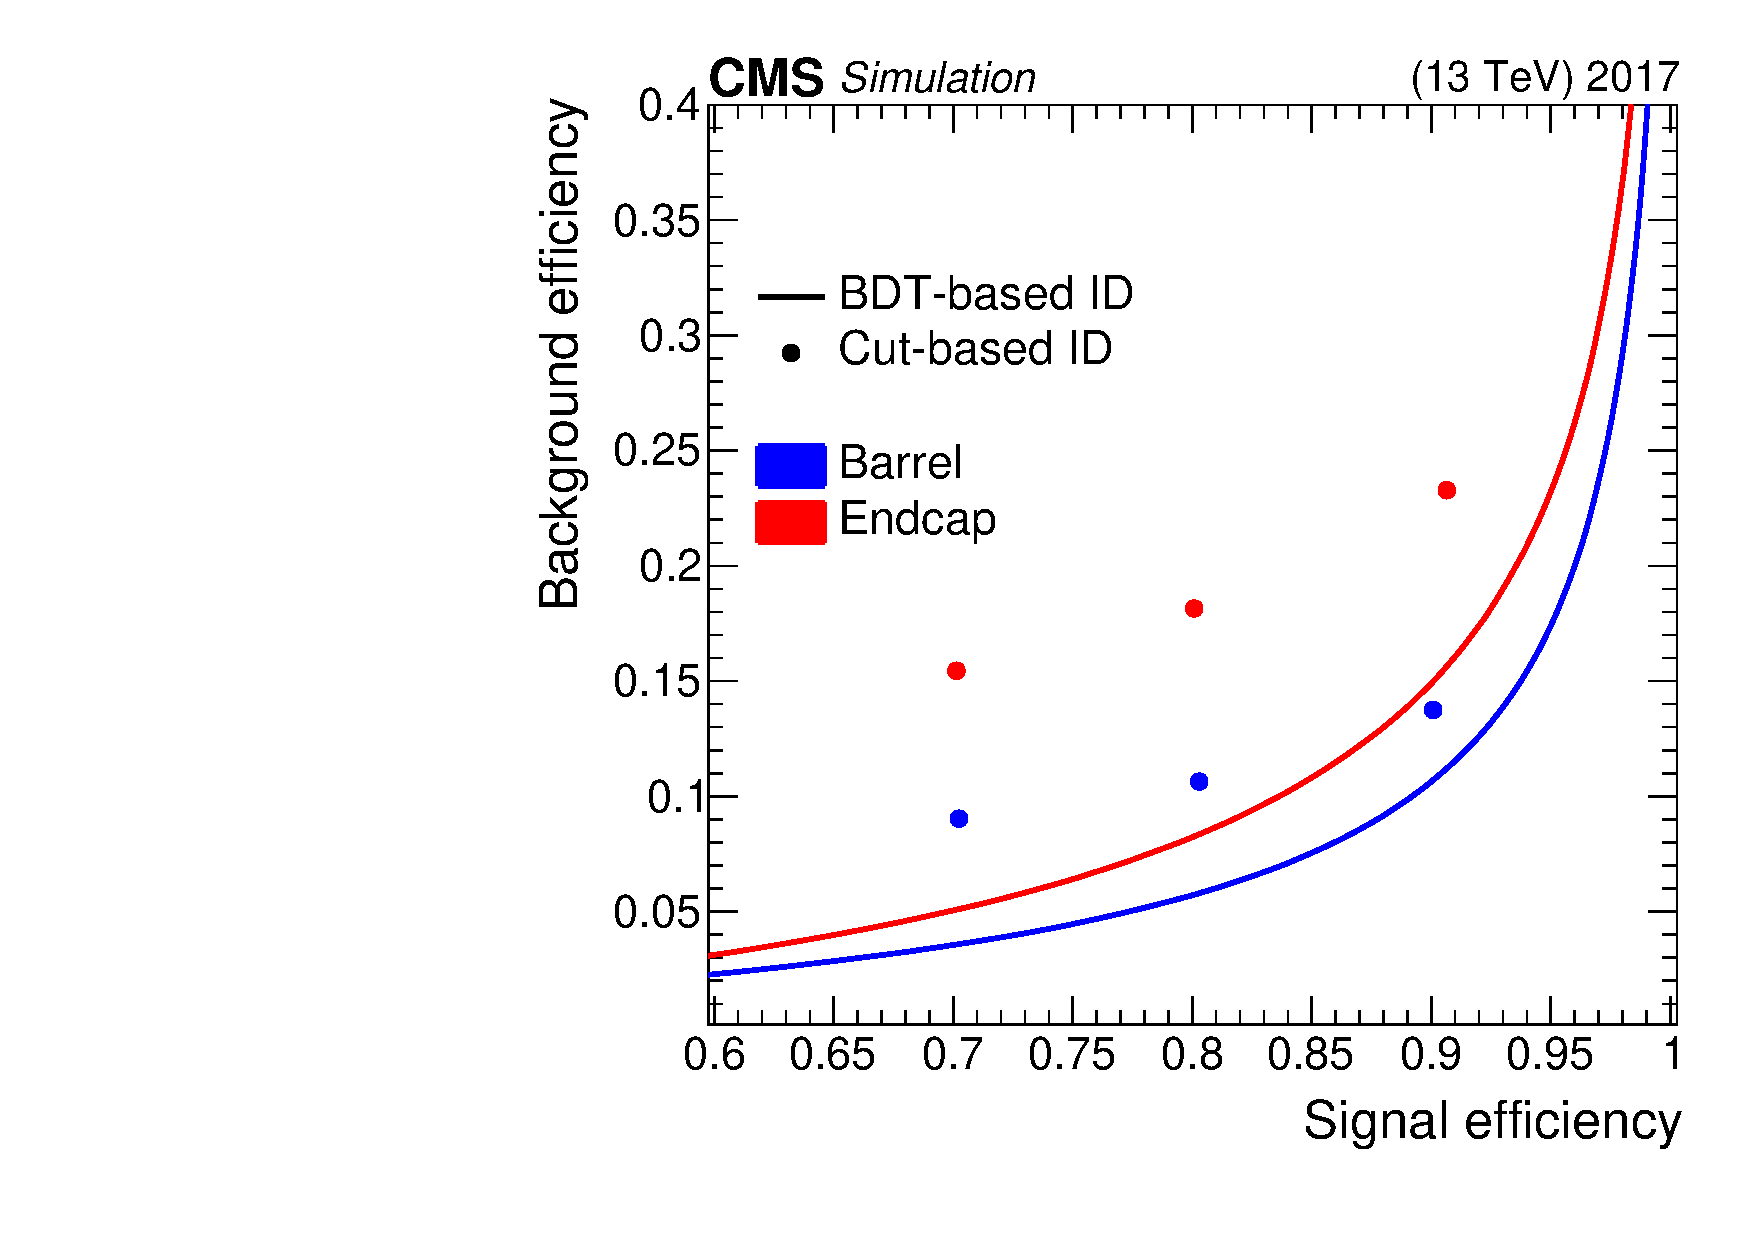
\includegraphics[width=0.49\textwidth]{Figures/Detector/CMS/photon_id_performance.pdf}
  \caption[Electron and Photon Identification Performance]{Performance of the electron (left) and photon (right) IDs in the ECAL barrel and endcaps evaluated for 2017 with simulated events. Different algorithms are shown for comparison's sake. For electrons, three algorithms are shown: a BDT trained without the isolation variables, the same BDT with isolation cuts applied separately, and a BDT with isolation variables included in training, where the last algorithm is the most performant. For photons, BDT-based and cut-based IDs are shown where the former is the most performant. Figures taken from Ref.~\cite{CMS:2020uim}.}\label{fig:eg_id_performance}
\end{figure}

The electron ID efficiencies are measured in data using $\PZ\rightarrow ee$ events. The photon ID efficiencies are also measured in $\PZ\rightarrow ee$ events, where the electrons are reconstructed in the same way as photons by omitting the information from the electron track. This is motivated by the fact that electrons and photons shower similarly in the ECAL and is validated using $\PZ\rightarrow\mu\mu\gamma$ events. The measured electron and photon ID efficiencies and a comparison to simulated efficiencies are shown for the WP90 working points in \cref{fig:eg_id_data_mc}. Scale factors are derived separately for each year and in bins of $\eta$ and \ET to correct the simulation to match data, and are up to 5\%~\cite{CMS:2020uim}. 

\begin{figure}
  \centering
  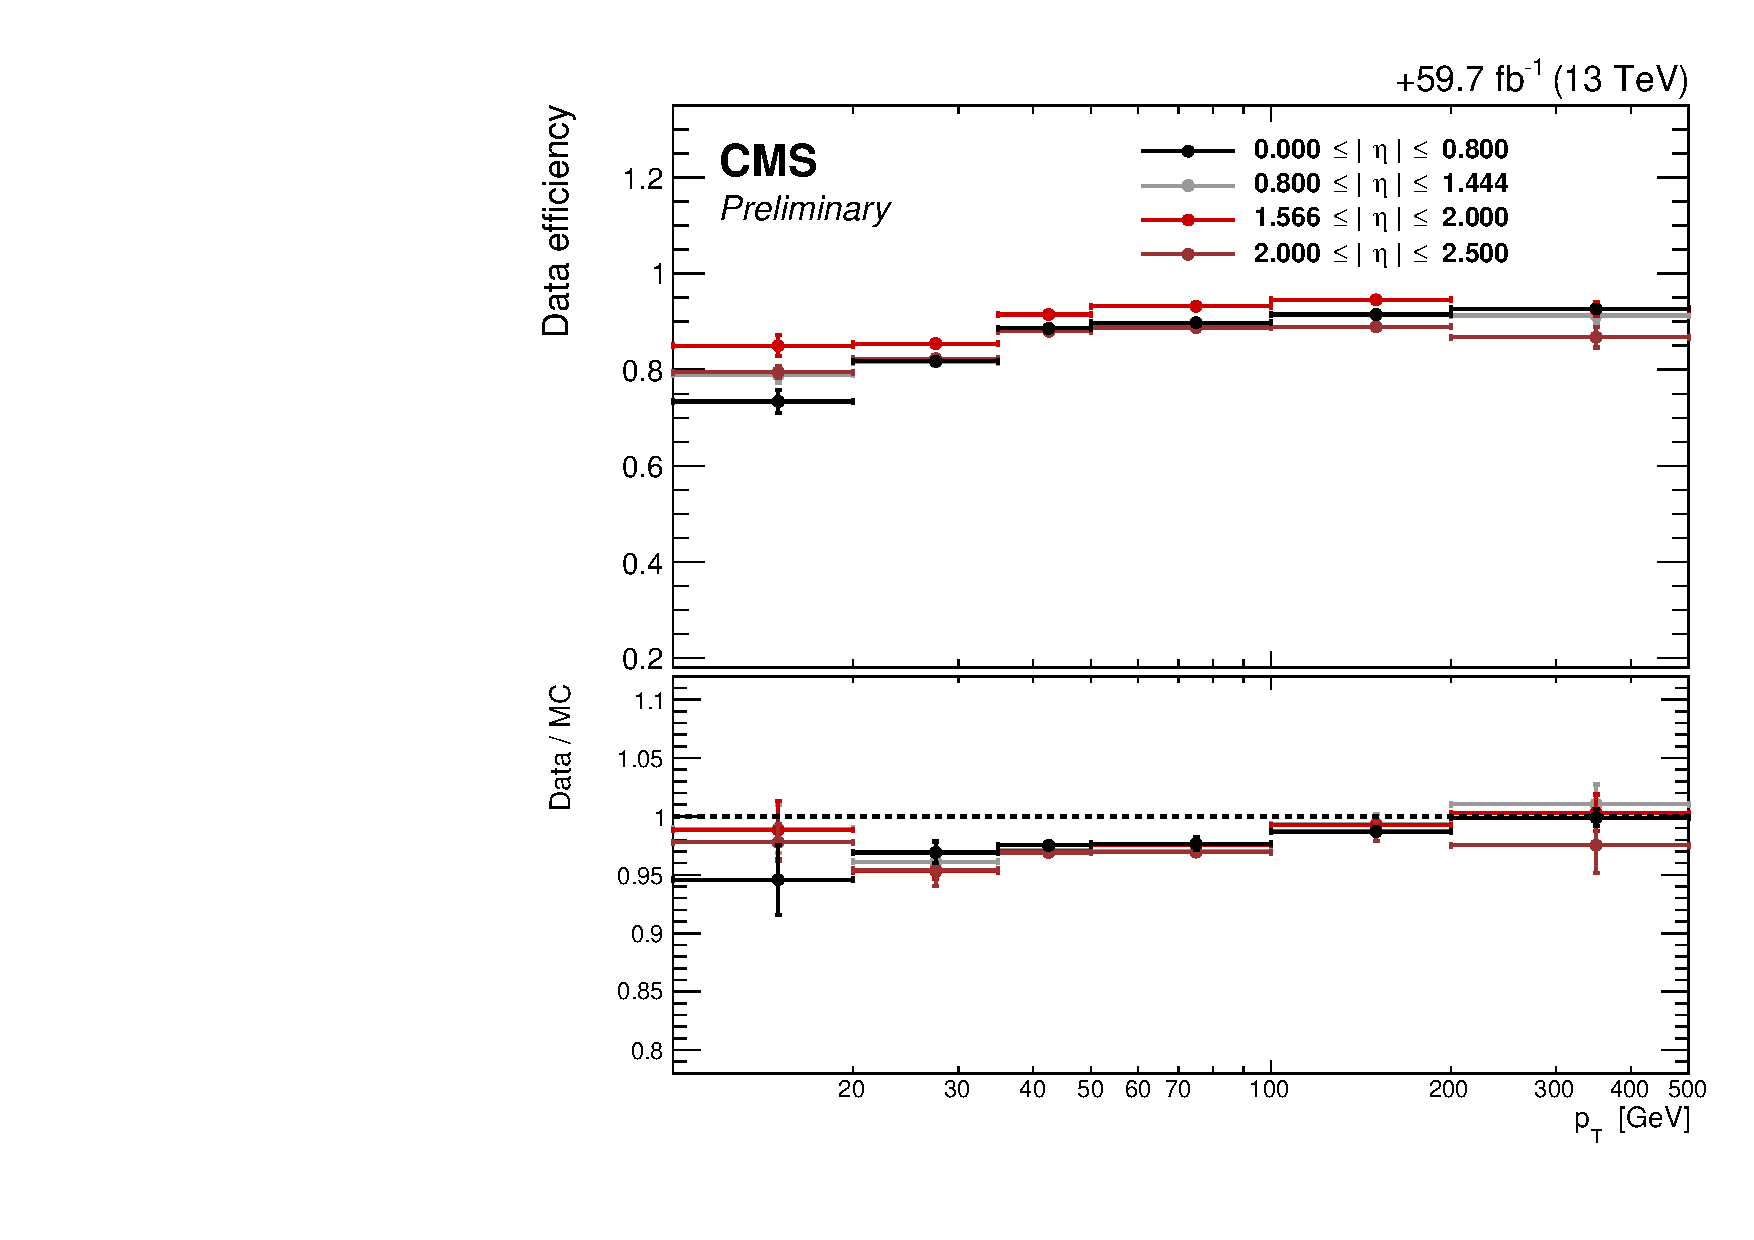
\includegraphics[width=0.60\textwidth]{Figures/Detector/CMS/electron_id_data_mc.pdf} \\
  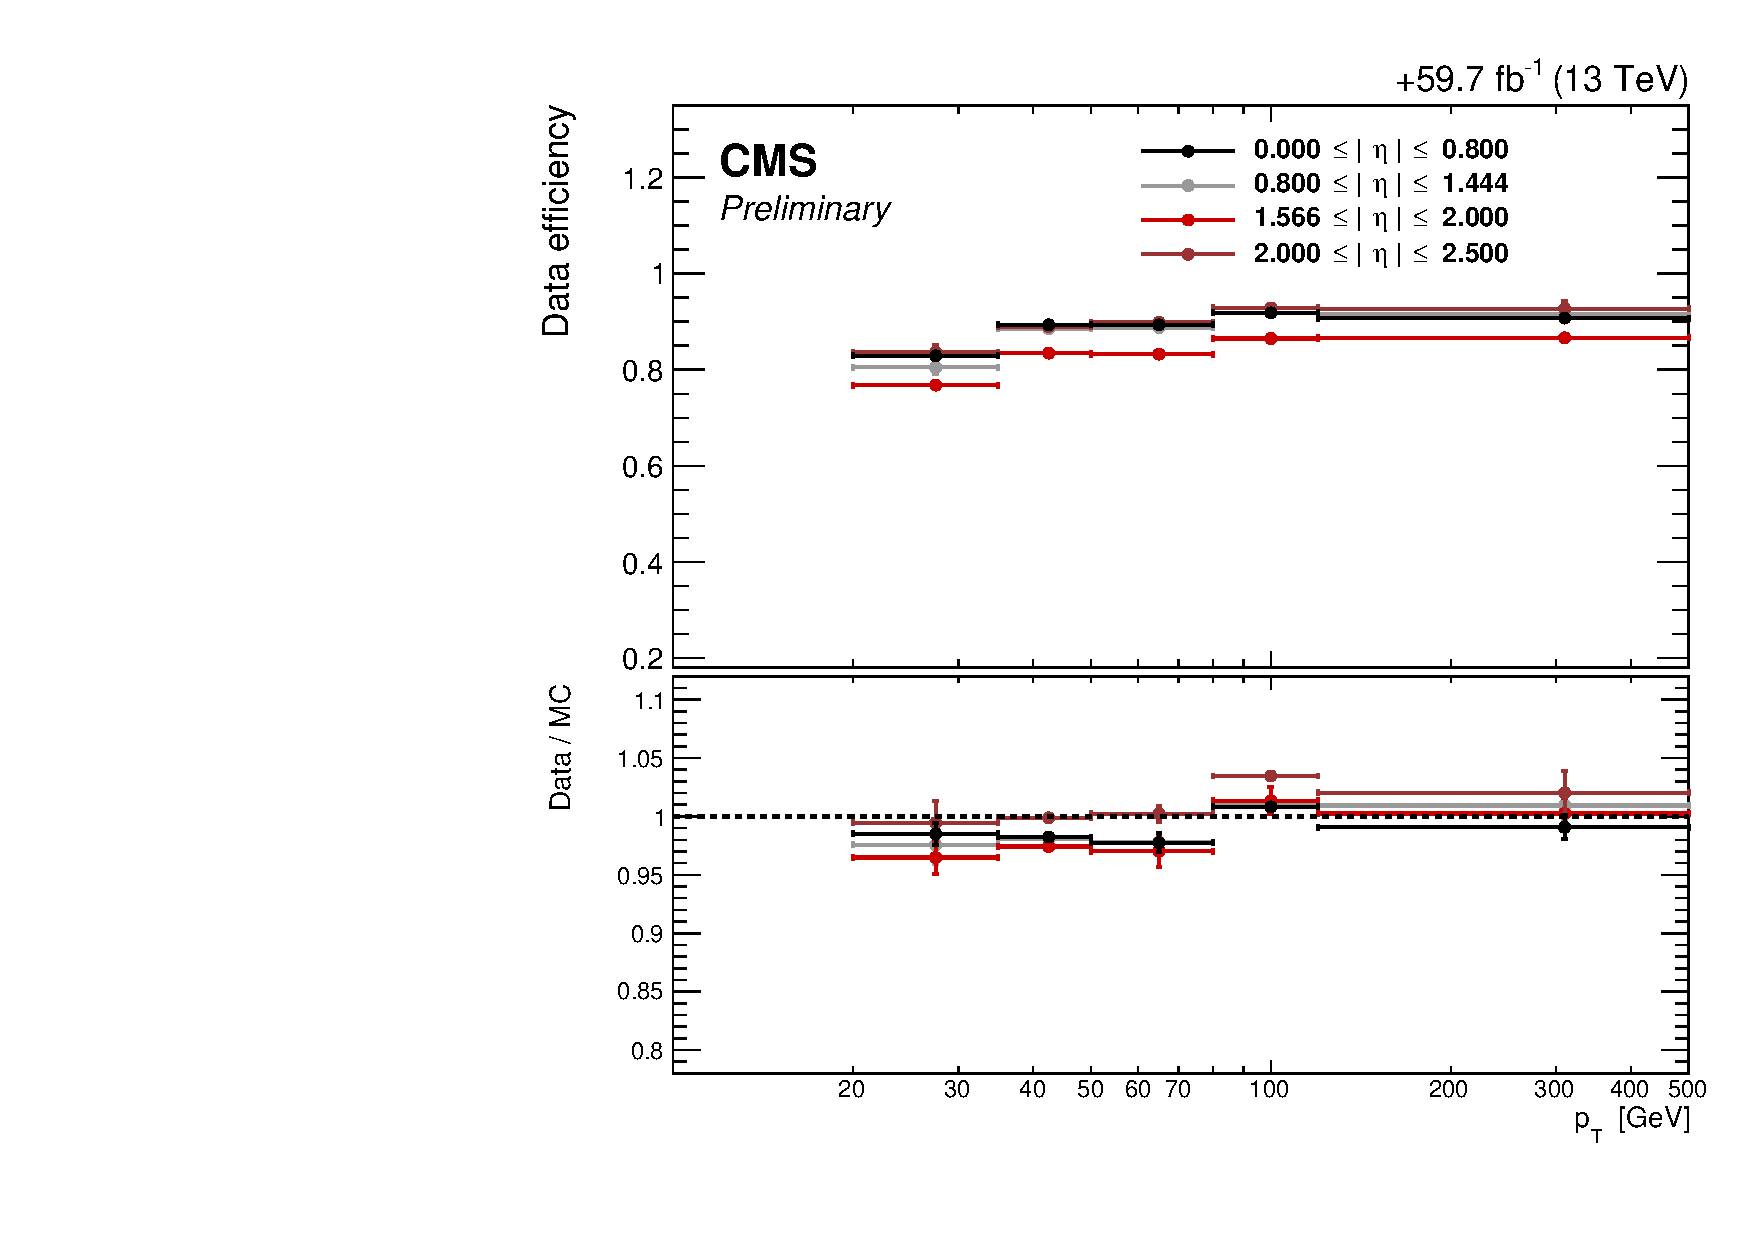
\includegraphics[width=0.60\textwidth]{Figures/Detector/CMS/photon_id_data_mc.pdf}
  \caption[Signal Efficiencies of Electron and Photon Identification Algorithms for the WP90 Working Point, Measured in Data and Simulation]{Signal efficiencies of the electron (top) and photon (bottom) BDT IDs at the WP90 working points. In the top halves of each figure, the efficiencies as measured in 2018 data with $\PZ\to ee$ events are shown. In the bottom halves, the ratio of the efficiencies in data to simulation (scale factors) are shown. The vertical error bars indicate combined statistical and systematic uncertainties. Figures taken from Ref.~\cite{CMS:2020uim}.}\label{fig:eg_id_data_mc}
\end{figure}

Finally, when searching for photon candidates, a conversion-safe electron veto (CSEV) can be used~\cite{CMS:2015myp}. This veto requires that there are no charged-particles tracks pointing to the photon SC, where the tracks are required to have a hit in the first layer of the pixel detector, and are not matched to a reconstructed conversion vertex. This leads to photon and electron efficiencies of about 99\% and 5\% for the barrel, and 98\% and 20\% for the endcap respectively. An even more stringent veto, the \textit{pixel veto}, rejects any photon where there exists at least two pixel hits that form a track pointing to the SC. This leads to photon and electron efficiencies of about 95\% and 1\% for the barrel, and 80\% and 5\% for the endcap respectively~\cite{CMS:2015myp}. In a similar fashion to the ID efficiencies, the veto efficiencies are measured in data using $\PZ\to\mu\mu\gamma$ events for photons, and $\PZ\to ee$ events for electrons and scale factors are used to correct the simulation.

\subsubsection{Energy Calibration}\label{sec:eg_energy_calibration}

The energy deposited in an ECAL crystal, $E_i$, is given by the following equation~\cite{CMS:2024ppo}:
\begin{equation}
  E_i = G \cdot LC_i(t) \cdot C_i \cdot A_i
\end{equation}
where:
\begin{itemize}
  \item $A_i$ is the pulse amplitude in ADC (analogue-to-digital converter) counts,
  \item $G$ are global factors that convert ADC counts to GeV,
  \item $C_i$ are intercalibration coefficients that account for differences between individual crystal's light-yield and photodetector response,
  \item and $LC_i(t)$ are time-dependent corrections due to radiation-induced response changes to the crystals.
\end{itemize}
The derivation of these corrections is described in Refs.~\cite{CMS:2013lxn,CMS:2024ppo}. The reconstructed energy of a supercluster, $E_{\text{SC}}$, is typically lower than the true energy, $E_{\text{true}}$, of the originating electron and photon due to imperfect containment of a shower, energy loss in the tracker material, and the application of thresholds when forming clusters. To correct this, simulated events with photons and electrons are studied and the distribution of $E_{\text{true}}/E_{\text{SC}}$ is parameterized by a Double Crystal Ball (DCB) function, which is an extension of the Crystal Ball function~\cite{Oreglia:1980cs} with power law tails on both sides. A multivariate regressor is used to fit the DCB shape parameters as functions of the shower shape variables, H/E, and the supercluster's uncorrected energy and position in the detector~\cite{CMS:2014afl}. Then, for a given supercluster, the energy is corrected by the mean of the Gaussian core of the DCB function, and the energy resolution is given by the width of the Gaussian core. Separate regressions are trained for electrons and photons to account for the small differences in how they shower.

For electrons with energies less than 200\GeV, the supercluster energy is combined with the momentum of the GSF track to improve the energy resolution. The combined energy measurement, $E_{\text{combined}}$ is given by:
\begin{equation}
  E_{\text{combined}} = \frac{E_{\text{ECAL}} / \sigma_E^2 + p_{\text{GSF}} / \sigma_p^2}{1 / \sigma_E^2 + 1 / \sigma_p^2}
  \label{eq:electron_combined_energy}
\end{equation}
where $E_{\text{ECAL}}$ is the regression-corrected supercluster energy, $p_{\text{GSF}}$ is the momentum of the GSF track, and $\sigma_E$ and $\sigma_p$ are the energy and momentum resolutions respectively. A final regression is applied to correct $E_{\text{combined}}$ which uses the inputs to \cref{eq:electron_combined_energy} as well as additional tracker quantities~\cite{CMS:2020uim}. The distribution of $E_{\text{true}}/E_{\text{combined}}$ before and after the energy corrections, and after the combination with the track momentum is shown in \cref{fig:ecal_regression_performance} for electrons in 2016 simulated events. After corrections, the distribution is centred around 1, and the width is reduced, indicating that the energy is corrected, and the resolution is improved. The resolution improves further after the combination with the track momentum. The distributions before the combination with the track momentum are indicative of those for photons. 

\begin{figure}
  \centering
  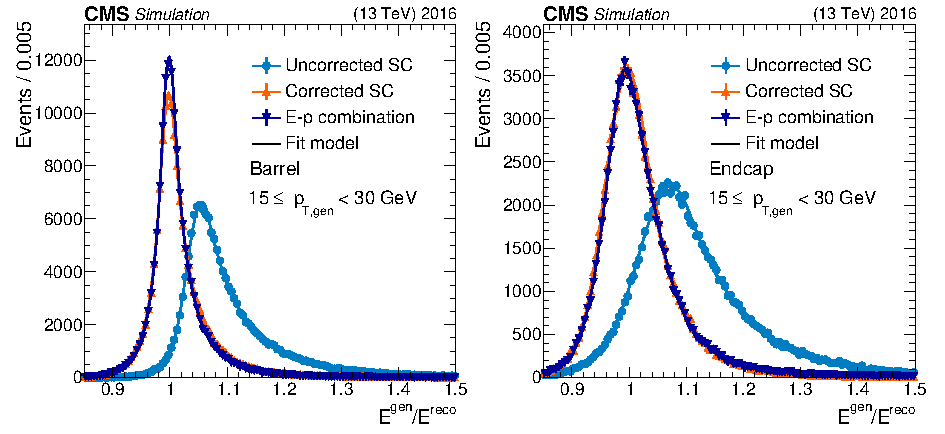
\includegraphics[width=\textwidth]{Figures/Detector/CMS/ecal_regression_performance.pdf}
  \caption[Electron Energy Corrections]{Ratio of the true to the reconstructed electron energy for $15 < \pt < 30$\GeV with and without regression corrections, and before and after the combination of the ECAL and tracker measurements, with a DCB function fit overlaid, in 2016 simulated events for barrel (left) and endcap (right) electrons. Vertical bars on the markers represent statistical uncertainties. Figure taken from Ref.~\cite{CMS:2020uim}.}\label{fig:ecal_regression_performance}
\end{figure}

After these simulation-based corrections, there are differences between data and simulation in the energy scales and resolutions of \eg objects. Further corrections are applied to correct the energy scale in data to match simulation, and since the resolution in simulation is better than that in data, smearings are applied to the simulation to match the data~\cite{CMS:2020uim}. These corrections are derived with $\PZ\rightarrow ee$ events by comparing the distribution of the invariant mass of the $\PZ$ boson in data and simulation. This is done in several stages. 

In the first stage, energy scale corrections are derived in about 18 hour intervals and in bins of $\eta$ corresponding to $0 < \abs{\eta} < 1$, $1.00 < \abs{\eta} < 1.44$, $1.57 < \abs{\eta} < 2.00$ and $2.00 < \abs{\eta} < 2.50$. The region, $1.44 < \abs{\eta} < 1.57$ represents the transition between the barrel and endcap regions and is not used. These initial corrections account for long-term drifts in the energy scale and accounts for $\eta$-dependent radiation damage. In the second stage, the energy scale and resolution is corrected in 50 categories, corresponding to 5 bins of $\eta$ and 10 bins of \RNINE. The magnitude of these corrections is up to 1.5\% and the systematic uncertainty associated with them is 0.05--0.1 (0.1--0.3)\% in the EB (EE), depending on the \RNINE bin~\cite{CMS:2020uim}. 

The final agreement between data and simulation in $Z\rightarrow ee$ events is shown in \cref{fig:zee_after_corrections} in two representative categories. The final energy resolution is found to be 2--5\%, depending on the $\eta$ and \RNINE of the electron~\cite{CMS:2020uim}. 

\begin{figure}
  \centering
  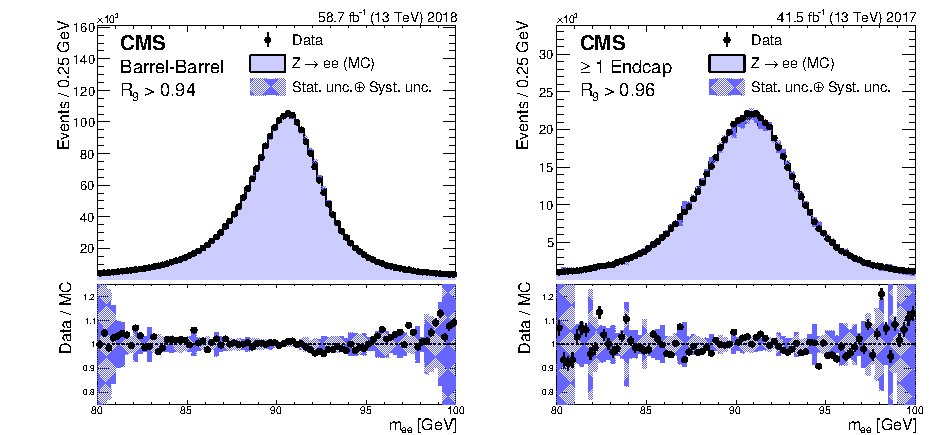
\includegraphics[width=\textwidth]{Figures/Detector/CMS/zee_after_corrections.pdf}
  \caption[Electron Energy Scale Agreement Between Simulation and Data]{Invariant mass distribution of the \PZ boson in $\PZ\to ee$ events, after scale and smearing corrections. Results are shown for barrel (left) and endcap (right) electrons in high \RNINE categories. The vertical bars on the markers represent the statistical uncertainties in data and the hatched regions show the combined statistical and systematic uncertainties in the simulation. The lower panels display the ratio of the data to the simulation with the bands representing the uncertainties in the simulation. Figure taken from Ref.~\cite{CMS:2020uim}.}\label{fig:zee_after_corrections}
\end{figure}